\documentclass[12pt,onecolumn,a4paper]{article}
\usepackage{epsfig,graphicx,amsthm,amsmath}
\usepackage{color,xcolor}
\usepackage{pgfplots}
\pgfplotsset{compat=newest}
\usepackage{tikz}
\usepackage{caption}
\usepackage{subcaption}
\usepackage{multirow}
\usepackage{xepersian}
\settextfont{XB Zar}
\setlatintextfont{Times New Roman}

\newtheorem{theorem}{قضیه}[section]
\newtheorem{corollary}{نتیجه‌}[theorem]

\pgfplotstableread[col sep = comma]{gibbs.csv}\gibbs
\pgfplotstableread{
-1 0
-1 -1
0 -1
0 1
1 1
1 0
}\gibbsref

\begin{document}
\title{توجیه وجود مثال‌های خصمانه \\ و انتقال‌پذیری آن‌ها} 
\author{رامین براتی}
\date{\today}
\maketitle

\begin{abstract}
چکیده
\end{abstract}

\section{مقدمه} 
مقدمه.

\section{کارهای مرتبط}
تاکنون، برای وجود مثال‌های خصمانه سه دلیل ارائه شده است. اولین دیدگاه توسط سجدی و همکاران
(مقاله)
مطرح شد. این دیدگاه، که با نام دیدگاه پاکت‌های نادر شناخته می‌شود، به شرح زیر است. در این دیدگاه، دلیل وجودی مثال‌های خصمانه وجود پاکت‌هایی در فضای ورودی شبکه هستند که احتمال مشاهده‌ی آنها بسیار کم است و شبکه در آن نواحی خروجی مناسبی نمی‌دهد. در این دیدگاه رابطه‌ی مثال‌های خصمانه با فضای ورودی شبکه را مشابه رابطه‌ی میان اعداد گویا و اعداد حقیقی می‌دانند. به این معنی که، احتمال گویا بودن یک نمونه‌ی تصادفی از یک بازه از اعداد حقیقی صفر است، با این وجود در همسایگی هر عدد حقیقی عددی گویا یافت می‌شود. با این حال،
همان گونه که در
(مقاله)
نیز به آن اشاره شده است، دلیل محکمی برای نشان دادن چنین رفتاری توسط شبکه ارائه نشده است و صرفا به مرتبط کردن آن به بسیار غیرخطی بودن نمایش یادگیری شده توسط شبکه اکتفا شده است. این دیدگاه چگونگی انتقال این مثال‌ها به شبکه‌های دیگر را نیز مشخص نمی‌کند.

دیدگاه دوم توسط گودفلو و همکاران
(مقاله)
مطرح شده است. این دیدگاه، که با نام دیدگاه خطی بودن شناخته می‌شود، هم اکنون مقبول‌ترین دیدگاهی است که در این زمینه ارائه شده است. طبق این دیدگاه، پدیده‌ی مثال‌های خصمانه در طبقه‌بندهای خطی در ابعاد بالا ظهور می‌کند و دلیل مشاهده‌ی این پدیده در شبکه‌های عصبی نیز مرتبط با علاقه‌ی ما در استفاده از الگوهای خطی در مدلسازی و آموزش این شبکه‌ها می‌باشد. گودفلو و همکاران با استفاده از این دیدگاه حمله‌ی
\lr{FGSM}
را طراحی کردند که از این خطی بودن شبکه‌های عصبی برای تولید مثال‌های خصمانه استفاده می‌کند. ضرب داخلی بین یک بردار وزن $w$ و یک مثال خصمانه‌ی $\tilde{x}=x+\eta$ را در نظر بگیرید.
\begin{equation*}
w^T\tilde{x}=w^Tx+w^T\eta
\end{equation*}
طبق معادله، اگر $\eta$ را برابر با $\mathrm{sign}(w)$ در نظر بگیریم، بیشترین تغییر را، تحت قید نورم ماکزیموم، در خروجی اعمال کرده‌ایم. خطی بودن به این معناست که شبکه رفتاری مشابه از خود نشان داده و در صورتی که $\eta$ را برابر با علامت گرادیان تابع هزینه در نقطه‌ی $x$ قرار دهیم، شبکه در طبقه‌بندی دچار خطا خواهد شد.

طبق این دیدگاه، دلیل انتقال مثال‌های خصمانه به دیگر شبکه‌ها، همگرایی این مدل‌ها به طبقه‌بند خطی بهینه است. دیدگاه خطی بودن دو پیش بینی مستقیم دارد، اول این که تمامی طبقه‌بندهای خطی از پدیده‌ی مثال‌های خصمانه رنج می‌برند و دوم این که اثر خطی بودن با افزایش ابعاد مسئله تشدید می‌شود. با این وجود، در
(مقاله)
هر دوی این پیش‌بینی‌ها زیر سوال می‌روند. ابتدا مسئله‌ای  مصنوع را در نظر می‌گیرند که برای آن طبقه‌بندی خطی وجود دارد که از مثال‌های خصمانه آزاد است و در ادامه نشان می‌دهند که در یک مسئله‌ی واقعی نیز با افزایش ابعاد قدرت مثال‌های خصمانه تشدید نمی‌شود.

دیدگاه سوم توسط تانای و همکاران
(مقاله)
 و با نام دیدگاه کجی مرز ارائه شده است. این دیدگاه برای طبقه‌بندهای خطی پیشنهاد شده و ظهور آن در شبکه‌های عصبی را منتج از شکلی غیرخطی از این پدیده می‌دانند. یک مسئله‌ی طبقه‌بندی دو کلاسی را در نظر بگیرید که برای آن یک طبقه‌بند خطی را آموزش داده‌ایم. این طبقه‌بند خطی یک مرز تصمیم
 $c$
 برای جدا کردن دو کلاس می‌یابد. حال طبقه‌بند بهینه‌ای را برای همان مسئله در نظر بگیرید که توسط مرکزهای دو کلاس تعریف شده باشد. این طبقه‌بند نیز یک مرز تصمیم
 $c^*$
 برای جدا کردن دو کلاس تعریف می‌کند. طبق دیدگاه کجی مرز در صورتی که مرز
 $c$
 با
 $c^*$
 زاویه داشته باشد، برای طبقه‌بند مثال‌های خصمانه وجود خواهد داشت. تانای و همکاران در ادامه نشان می‌دهند که می‌توان زاویه‌ی بین دو مرز را با منظم کردن\LTRfootnote{regularize}
طبقه‌بند کاهش داد. در پایان، تانای و همکاران با توجه به نوع و شکل اختلالات خصمانه‌ای که در شبکه‌های عصبی مشاهده می‌کنند، دلیل وجود مثال‌های خصمانه برای این شبکه‌ها را منظم نبودن این شبکه‌ها اعلام می‌کنند. با این که تانای و همکاران دلایل خوبی در تایید دیدگاه کجی مرز ارائه می‌دهند، چگونگی تعمیم آن به شبکه‌های عصبی و دیگر مدل‌های غیرخطی را مشخص نمی‌کنند. همچنین، در این دیدگاه دلیلی برای انتقال‌پذیری مثال‌های خصمانه ارائه نشده است.

همان گونه که مشاهده می‌شود، هیچ‌کدام از دیدگاه‌های مطرح شده توانایی توجیه و تشریح تمامی مشاهدات مرتبط با مثال‌های خصمانه را ندارند. با این حال، هرکدام بخش محدودی از مشاهدات را توجیه می‌کنند. در اینجا، دیدگاه جدیدی را مطرح می‌کنیم که توانایی توجیه وجود مثال‌های خصمانه و انتقال‌پذیری آن‌ها را دارد و  در عین حال، با مشاهداتی که توسط دیدگاه‌های قبلی مطرح شده نیز سازگازی دارد. در ادامه، این دیدگاه جدید را شرح می‌دهیم.

\section{پدیده‌ی رونگه و مثال‌های خصمانه}
در این بخش، دیدگاه جدیدی را در مورد دلیل وجود مثال‌های خصمانه و انتقال‌پذیری آن‌ها ارائه می‌دهیم. در این دیدگاه، مثال‌های خصمانه را اثر جانبی پدیده‌ی رونگه دانسته و انتقال‌پذیری آن‌ها را با استفاده از اصل داربو توجیه می‌کنیم. ابتدا پدیده‌ی رونگه را توصیف می‌کنیم.

در آنالیز عددی، پدیده‌ی رونگه مشکلی است که هنگام درون‌یابی با استفاده از چندجمله‌ای‌های درجه بالا به وجود می‌آید. طبق قضیه‌ی تقریب وایرشتراس\LTRfootnote{Weierstrass approximation theorem}،
هر تابع پیوسته‌ی 
$f(x)$
که بر روی یک بازه‌ی
$[a,b]$
تعریف شود را می‌توان با استفاده از یک چندجمله‌ای درون‌یاب
$P_n(x)$
تقریب زد. به عبارت دقیق‌تر
\begin{equation*}
    \lim_{n\rightarrow \infty}\left(\max _{{a\leq x\leq b}}\left|f(x)-P_{n}(x)\right|\right)=0.
\end{equation*}
طبق این قضیه، طبیعی است که انتظار داشته باشیم که با افزایش 
$n$
به تقریب دقیق‌تری از تابع مورد نظر دست یابیم. با این وجود، ممکن است که چندجمله‌ای‌هایی که انتخاب شده‌اند خاصیت همگرایی یکپارچه را نداشته باشند. توجه کنید که قضیه‌ی تقریب وایرشتراس فقط وجود این چندجمله‌ای را تضمین می‌کند، و مسیری برای یافتن این چندجمله‌ای مشخص نمی‌کند. در واقع، چندجمله‌ای‌هایی که به این صورت ساخته می‌شوند ممکن است با افزایش درجه‌ی چندجمله‌ای واگرا شوند. این مشکل به صورت الگوهای نوسانی بروز کرده که در نزدیکی نقاط درون‌یابی انتهایی بازه افزایش می‌یابد. شناسایی این پدیده را به  کارل رونگه\LTRfootnote{Carl David Tolme Runge}،
ریاضیدان آلمانی، منتصب می‌کنند.

تابع رونگه با تعریف 
$f(x)=\frac{1}{1+25x^2}$ 
را در نظر بگیرید. چندجمله‌ای درون‌یاب این تابع را با استفاده از نقاط 
$x_i$ 
تعریف می‌کنیم، به طوری که
$x_{i}=\frac{2i}{n}-1$ 
و 
$i\in \left\{0,1,\dots ,n\right\}$.
همان گونه که مشاهده می‌شود، نقاط 
$x_i$ 
در بازه‌ی 
$[-1,1]$ 
و با فاصله‌ی یکسان توزیع شده‌اند. رونگه متوجه شد که چندجمله‌ای درون‌یابی که به روش ذکر شده ساخته شود، در نزدیکی مرز‌های دامنه‌ی تابع نوسان می‌کند. حتی می‌توان نشان داد که خطای درون‌یابی با افزایش 
$n$ 
 به صورت بیکران افرایش می‌یابد.

پدیده‌ی رونگه هنگام درون‌یابی با استفاده از پایه‌های تک‌جمله‌ای\LTRfootnote{Monomial basis} 
بروز پیدا می‌کند. با این حال تغییر این توابع پایه برای حل مسئله کافی نیست. اگر از توابع پایه‌ی مثلثاتی، مثلا توابع پایه‌ی چبیشف، برای تشکیل چندجمله‌ای درون‌یاب استفاده کنیم، با مشکل مشابهی مواجه می‌شویم. این مشکل  با نام پدیده‌ی گیبس\LTRfootnote{Gibbs phenomenon}
شناخته می‌شود. پدیده‌ی گیبس باعث به وجود آمدن نوساناتی در نزدیکی ناپیوستگی‌های تابع شده و این امر موجب فراجهش
\LTRfootnote{overshoot} 
در این نقاط می‌شود. در شکل 
\ref{fig:runge_gibbs} 
این دو پدیده با مثال‌هایی نشان داده‌ شده‌اند.

 \begin{figure}
    \centering
    \begin{subfigure}[b]{0.45\textwidth}
        \centering
        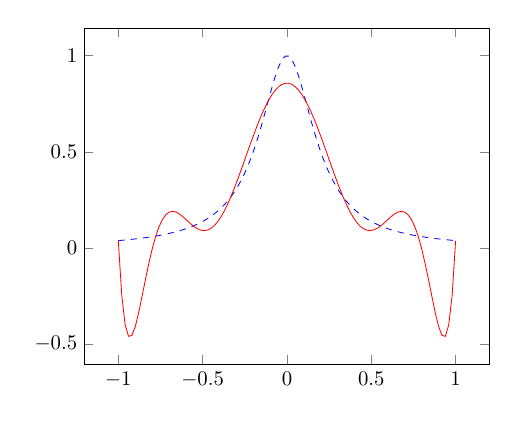
\begin{tikzpicture}[scale=0.75]
            \begin{axis}[xmin=-1,xmax=1,xmin=-1.2,xmax=1.2,samples=100]
                \addplot[domain=-1:1,blue,dashed]{1/(1+25*x*x)};
                \addplot[domain=-1:1,red,solid]{16.545674722429712 * x*x*x*x*x*x*x*x*x*x + 8.851286807773627e-13 * x*x*x*x*x*x*x*x*x + -12.079377458718012 * x*x*x*x*x*x*x*x + -1.6319051537287015e-12 * x*x*x*x*x*x*x + -22.778903788331114 * x*x*x*x*x*x + 8.747268893200492e-13 * x*x*x*x*x + 25.348331583973515 * x*x*x*x + -1.4087385060936399e-13 * x*x*x + -7.854564043148674 * x*x + 6.6005027351349585e-15 * x + 0.8573005222561162};
            \end{axis}
         \end{tikzpicture}
        \caption{پدیده‌ی رونگه}
        \label{fig:runge}
    \end{subfigure}
    \hfill
    \begin{subfigure}[b]{0.45\textwidth}
        \centering
        \begin{tikzpicture}[scale=0.75]
            \begin{axis}[xmin=-1,xmax=1,xmin=-1.2,xmax=1.2,samples=100]
                \addplot[mark=none,blue,dashed] table{\gibbsref};
                \addplot[mark=none,red,solid] table{\gibbs};
            \end{axis}
         \end{tikzpicture}
        \caption{پدیده‌ی گیبس}
        \label{fig:gibbs}
    \end{subfigure}
       \caption{دو پدیده‌ی رونگه و گیبس. در هر دو نمودار خم آبی تابع هدف و خم قرمز تقریب متناظر با آن تابع می‌باشد. (آ) تابع رونگه و تقریب آن توسط یک چندجمله‌ای درجه 10. (ب) تابع پله‌ای و تقریب آن با استفاده از 30 جمله‌ی اول سری فوریه‌ی متناظر آن.}
       \label{fig:runge_gibbs}
\end{figure}

همان گونه که در شکل نیز مشاهده می‌شود، پدیده‌ی رونگه تاثیر به مراتب مخرب‌تری از پدیده‌ی گیبس دارد. در واقع، می‌توان نشان داد که خطای درون‌یابی  در مثال بالا برابر با 
$O(2^n‌)$ 
است، در حالی که خطایی که پدیده‌ی گیبس در محاسبات وارد می‌کند 
$O(1)$ 
است. در پدیده‌ی رونگه، همان طور که قبلا نیز به آن اشاره شد، بیشترین میزان خطا در نزدیکی مرزهای دامنه‌ی ورودی تابع اتفاق می‌افتد. به عبارت دیگر، اگر دامنه‌ی ورودی بازه‌ی 
$[-1,1]$ 
باشد، انتظار داریم ابعادی از ورودی که به مقادیر $1$ یا $-1$ نزدیک باشند بیشترین حساسیت را در خروجی تابع درون‌یاب به وجود بیاورند. در مقابل، در صورتی که با پدیده‌ی گیبس رو به رو باشیم، این حساسیت در قسمت‌هایی از سیگنال ورودی که ناپیوستگی وجود دارد به وجود می‌آید.

پدیده‌ی رونگه هنگام درون‌یابی با استفاده از چندجمله‌ای‌های درجه بالا بروز می‌کند. ولی اکثریت مدل‌های یادگیری ماشین، از جمله شبکه‌های عصبی، از پایه‌ی تک‌جمله‌ای درجه یک برای ورودی استفاده می‌کنند. با این وجود، این مدل‌ها به طرق مختلف برای یادگیری توابع غیرخطی تعمیم می‌یابند. در نتیجه، دور از ذهن نیست که پدیده‌ی رونگه، یا پدیده‌ی مشابهی، در این مدل‌ها وجود داشته باشد. برای محک زدن این ادعا، می‌توان آزمایش ساده‌ای طراحی کرد. در صورتی که با پدیده‌ی رونگه مواجه باشیم، تغییر تابع پایه‌ی تک‌جمله‌ای به پایه‌ی چبیشف، باید تاثیرات مشخصی در بهبود مقاومت شبکه در برابر حملات خصمانه و ماهیت این حملات داشته باشد. نتایج این آزمایش‌ها شواهد بسیار قویی در تایید ارتباط مثال‌های خصمانه و پدیده‌ی رونگه نشان می‌دهند. جزییات و نتایج این آزمایش‌ها را در بخشی جداگانه شرح و بسط می‌دهیم.

با توجه به اینکه بهبود مشاهده شده بدون تغییر در تابع هدف، روش آموزش یا تغییر فاکتور غیرخطی حاصل شده، دور از ذهن نیست که انتقال‌پذیری مثال‌های خصمانه حاصل از اصل داربو باشد. ابتدا اصل داربو را آن طور که در (کتاب) آمده بیان می‌کنیم.
\begin{theorem}[اصل داربو]
    در تمامی انواع بسط طیفی (از جمله سری‌های توانی عادی)، هم دامنه‌ی همگرایی در صفحه مختلط و هم نرخ همگرایی توسط مکان و قدرت بدترین تکینگی در صفحه‌ی مختلط تعیین می‌شود. در اینجا، منظور از تکینگی قطب‌ها، توان‌های کسری، لوگاریتم‌ها و دیگر نقاط شاخه و ناپیوستگی‌های تابع 
    $f(z)$ 
    یا هرکدام از مشتقات آن است.
\end{theorem}

از اصل داربو می‌توان قضیه‌ی فرعی زیر را مستقیما نتیجه گرفت.

\begin{corollary}
    اگر دو تابع 
    $f(z)$ 
    و 
    $g(z)$ 
    دارای تکینگی‌های یکسان محدود کننده‌ی همگرایی باشند، ضرایب مجانب بسط طیفی آن‌ها در حد
    $n \rightarrow \infty$ 
    برابر خواهد بود.
\end{corollary}

همان گونه که در (مقاله) ذکر شده است، مثال‌های خصمانه‌ی یک شبکه را می‌توان به شبکه‌ی دیگری که بر روی داده‌های آموزشی متفاوتی آموزش داده شده است منتقل کرد. با توجه به نتیجه‌ی مستقیم اصل داربو، انتقال‌پذیری مثال‌های خصمانه را می‌توان به وجود تکینگی‌ها در تابعی که قصد یادگیری آن را داریم نسبت داد. این موضوع توجیه قابل قبولی برای انتقال مثال‌های خصمانه بین شبکه‌های مختلف، که مستقل از داده‌های آموزشی استفاده شده است، ارائه می‌دهد. حال تعاریف لازم برای تشریح دلیل وجود مثال‌های خصمانه، چگونگی تاثیر آن‌ها بر خروجی شبکه و انتقال‌پذیری آن‌ها را داریم.

مثال‌های خصمانه نقاطی در همسایگی مثال‌های طبیعی در نزدیکی مرز دامنه‌ی ورودی شبکه هستند که خروجی شبکه در همسایگی این مثال‌ها نوسنات شدیدی ناشی از پدیده‌ی رونگه دارد. خطایی که با جا به جایی اتفاقی در همسایگی مثال طبیعی در ابعاد مختلف ایجاد می‌شود تاثیر هم را خنثی می‌کنند ولی با استفاده از اطلاعات گرادیان شبکه در آن نقطه، می‌توان مثالی در همسایگی آن مثال طبیعی یافت که شبکه با اطمینان بالایی آن را اشتباه طبقه‌بندی می‌کند.

به عبارت دیگر، اکثر مثال‌های طبیعی در نزدیکی یا روی مرز دامنه‌ی ورودی هستند\footnote{به عنوان مثال، در 
\lr{MNIST} 
اکثر ابعاد ورودی مقدار ۰ یا ۱ را دارند که دقیقا بر روی مرز دامنه‌ی ورودی قرار گرفته است.}.
این نواحی از دامنه‌ی همگرایی بسط طیفی یادگیری شده بیرون هستند و در نتیجه، خروجی تابع در این نواحی به شدت نوسان می‌کند. این مسئله، احتمالا در ابعاد بالا بسیار تشدید می‌شود، زیرا در ابعاد بالا اکثر جرم فضا در نوار نازکی پشت مرز دامنه‌ی ورودی قرار گرفته است. با توجه به این موضوع، محتمل است که وجود اختلالات خصمانه‌ی جهانی، که در (مقاله) مطرح شده‌اند، ناشی از این توزیع شدن مثال‌های طبیعی در نزدیکی مرزها و وجود تقارن در پدیده‌ی رونگه باشد.

از آنجایی که تعداد پارامترهای شبکه‌های عصبی بسیار زیاد است، با استفاده از اصل داربو، می‌توان انتظار داشت که ضرایب مجانب بسط طیفی یادگیری شده برای این شبکه‌ها بسیار نزدیک یا برابر باشد. در نتیجه، تمامی این شبکه‌ها، بدون در نظر گرفتن معماری و مجموعه‌ی آموزشی استفاده شده، رفتار یکسانی در اطراف تکینگی‌ها نشان می‌دهند و به همین دلیل مثال‌های خصمانه‌ای که برای یکی از این شبکه‌ها ساخته می‌شود برای بقیه‌ی شبکه‌ها نیز خصمانه است.

دیدگاه جدید توجیهی برای مقاوم شدن شبکه‌ها در برابر مثال‌های خصمانه با استفاده از آموزش خصمانه نیز ارائه می‌دهد. این یک واقعیت شناخته شده است که در صورتی که درون‌یابی را با استفاده از گره‌های چبیشف انجام دهیم، تاثیر پدیده‌ی رونگه کمینه خواهد شد. گره‌های چبیشف در نزدیکی مرز دامنه‌ی ورودی تراکم دارند. بر این اساس، دیدگاه پیشنهادی وجود آموزش خصمانه را پیش‌بینی می‌کند. طبق دیدگاه جدید، آموزش خصمانه‌ی شبکه تاثیری مانند استفاده از گره‌های چبیشف هنگام یافتن ضرایب بسط طیفی دارد.

دیدگاه پیشنهاد شده در توصیف پدیده‌ی مثال‌های خصمانه با دیدگاه‌های مطرح شده‌ی قبلی اشتراکاتی دارد. در دیدگاه جدید، پدیده‌ی مثال‌های خصمانه از بسیار غیرخطی بودن شبکه‌های عصبی نتیجه می‌شود و از این لحاظ با دیدگاه پاکت‌های نادر سازگار است. در مقابل، با اقتباس از مثال مجموعه‌های اعداد، در دیدگاه جدید مثال‌های خصمانه نقش اعداد حقیقی و مثال‌های طبیعی نقش اعداد صحیح را بازی می‌کنند. به این معنی که، مانند تابع رونگه، مقدار تقریب در نقاطی با مقدار مورد نظر برابر است ولی اگر کمی از این نقاط فاصله بگیریم خروجی تابع بی‌معنی خواهد بود.

در دیدگاه جدید، پدیده‌ی مثال‌های خصمانه و پدیده‌ی رونگه ارتباط تنگاتنگی دارند. پدیده‌ی رونگه به دلیل همگرا نشدن بسط  تیلور در بعضی نواحی به وجود می‌آید. در واقع، دیدگاه خطی بودن اثر جانبی محدود کردن بسط تیلور تابع به جمله‌ی خطی است. از این لحاظ، دیدگاه جدید نیز وجود حمله‌ی
\lr{FGSM}
را پیش‌بینی می‌کند. بسط تیلور تابع $f(x)$ حول مثال خصمانه‌ی $\tilde{x}=x+\eta$ به صورت زیر است.
\begin{equation*}
f(\tilde{x})=f(x)+\eta^T\nabla f(x) + O(\|\eta\|^2)
\end{equation*}
همان گونه که مشاهده می‌شود، در صورتی که $\eta$ را برابر $\mathrm{sign}(\nabla f(x))$ قرار دهیم، خروجی تابع بیشترین تغییر را، تحت قید نورم ماکزیموم، خواهد داشت. از آنجایی که شبکه‌ی عصبی تقریب ما از تابع $f$ است، می‌توانیم گرادیان شبکه را به عنوان جانشین گرادیان $f$ در نظر بگیریم. منتهی، به دلیل واگرا شدن بسط طیفی، این کار مقدار خروجی شبکه‌ی عصبی را به یک مقدار بی‌معنی تبدیل خواهد کرد. نکته‌ای که رابطه‌ی این دو دیدگاه را مشخص می‌کند، برابر بودن گرادیان تابع هزینه‌ی شبکه‌ی \lr{softmax} با گرادیان درایه‌ی متناظر با برچسب صحیح مثال طبیعی در خروجی شبکه‌ی عصبی است. همچنین، در دیدگاه جدید، دلیل انتقال‌پذیری مثال‌های خصمانه برابر شدن ضرایب مجانب بسط طیفی تمامی شبکه‌ها است که با توجیه مطرح شده توسط دیدگاه خطی بودن قرابت دارد.

از سه دیدگاه رقیب، شاید دورترین دیدگاه به دیدگاه پیشنهادی دیدگاه کجی مرز باشد. با این وجود، حتی در این جا نیز می‌توان ردپایی از اشتراکات را یافت. همان طور که گزارش شد، در دیدگاه کجی مرز، اصلی‌ترین راه برای کاهش اثرات پدیده‌ی مثال‌های خصمانه، منظم کردن شبکه عنوان شده است. از منظر راه حل، دیدگاه جدید هم بر منظم کردن شبکه تاکید دارد زیرا منظم کردن یکی از روش‌های کاهش تاثیرات پدیده‌ی رونگه نیز هست.

\section{شواهد و آزمایش‌ها}
در این بخش، شواهد فیزیکی در تایید رابطه‌ی پدیده‌ی مثال‌های خصمانه و پدیده‌ی رونگه را ارائه می‌دهیم. همان گونه که در بخش قبل به آن اشاره شد، پدیده‌ی رونگه هنگام درون‌یابی با استفاده از پایه‌های تک‌جمله‌ای به وجود می‌آید. در نتیجه، با تغییر پایه‌های مورد استفاده به توابع مثلثاتی از میان خواهد رفت. با این وجود، استفاده از توابع پایه‌ی مثلثاتی راه حل نهایی برای از میان بردن مثال‌های خصمانه نیست. در این صورت با پدیده‌ی گیبس مواجه خواهیم شد که مقیاس و شکل بسیار متفاوتی نسبت به پدیده‌ی رونگه دارد. پس از تغییر توابع پایه‌ انتظار داریم که دو چیز مشاهده کنیم. اول، از آنجایی که خطایی که پدیده‌ی گیبس در محاسبات وارد می‌کند کران‌دار است، انتظار داریم این تغییر تفاوت معنی داری در نرخ موفقیت حملات بگذارد. دوم، پدیده‌ی گیبس تاثیر خود را در ناپیوستگی‌های سیگنال ورودی نشان می‌دهد در حالی که حساسیت به وجود آمده توسط پدیده‌ی رونگه خود را در مرزها نشان می‌دهد. به عبارت دیگر، اگر فضای ورودی را تصویر سطح خاکستری در نظر بگیریم، پدیده‌ی گیبس موجب به وجود آمدن حساسیت در لبه‌های تصویر می‌شود ولی پدیده‌ی رونگه در ابعادی که به مقادیر انتهایی بازه‌ی ورودی نزدیک‌اند حساسیت ایجاد می‌کند.

برای این آزمایش سه مدل را برای آموزش بر روی
\lr{MNIST}
در نظر می‌گیریم. هر کدام از مدل‌ها را با استفاده از پایه‌های تک‌جمله‌ای $x$ و چبیشف $\cos(\pi x)$ آموزش می‌دهیم. استفاده از توابع پایه‌ی تک‌جمله‌ای معادل استفاده از لایه‌ی ورودی عادی و استفاده از توابع چبیشف معادل اعمال تبدیل $\cos(\pi x)$ در لایه‌ی ورودی می‌باشد. سپس به هر مدل با استفاده از روش
\lr{FGSM}
حمله کرده و  دقت مدل قبل و بعد از حمله را ثبت کردیم. برای انجام حمله از پیاده‌سازی موجود در کتابخانه‌ی \lr{cleverhans} استفاده شد. این آزمایش را برای هر مدل ده بار تکرار کردیم. نتایج در جدول
\ref{tbl:sizes}
گزارش شده است. همان گونه که مشاهده می‌شود، نتایج آزمایش پیش‌بینی دیدگاه پیشنهادی را تایید می‌کند.

\begin{table}[]
    \begin{latin}
    \resizebox{\linewidth}{!}{
    \begin{tabular}{|l|l|l|l|l|l|}
        \hline
        \multirow{2}{*}{Model} & \multirow{2}{*}{Size}              & \multicolumn{2}{l|}{Monomial}     & \multicolumn{2}{l|}{Chebyshev}           \\ \cline{3-6} 
                               &                                    & Clean Acc.     & Adversarial Acc. & Clean Acc.     & Adversarial Acc.        \\ \hline
        Perceptron               & $784\times10$                      & $92.39\pm0.07$ & $3.99\pm0.04$    & $91.83\pm0.18$ & $\mathbf{33.84\pm1.69}$ \\ \hline
        FC                     & $784\times 200\times 200\times 10$ & $97.76\pm0.08$ & $1.16\pm0.100$   & $97.25\pm0.24$ & $\mathbf{51.05\pm1.85}$ \\ \hline
        CNN                    & $784\times 200\times 200\times 10$ & $99.21\pm0.20$ & $4.14\pm1.61$    & $99.03\pm0.12$ & $\mathbf{66.07\pm3.11}$ \\ \hline
    \end{tabular}
    }
    \end{latin}
    \caption{مدل‌های استفاده شده در آزمایش، ابعاد آنها و دقت آنها قبل و پس از حمله‌ی \lr{FGSM}. همان طور که مشاهده می‌شود، استفاده از توابع پایه‌ی چبیشف به صورت معنی داری باعث بهبود مقاومت در برابر حمله می‌شود.}
    \label{tbl:sizes}
\end{table}
با این وجود نکته‌ای در نتایج این آزمایش جلب توجه می‌کند. مطابق پیش‌بینی دیدگاه پیشنهادی، مقاومت در برابر مثال‌های خصمانه با بیشتر شدن تعداد ضرایب در مدل‌های \lr{Perceptron} و \lr{FC} تک‌جمله‌ای کاهش می‌یابد. با این وجود، در مدل \lr{CNN} این روند معکوس می‌شود. این موضوع نشان می‌دهد که استفاده از لایه‌ی کانولوشن تاثیری در پدیده‌ی مثال‌های خصمانه دارد که در دیدگاه پیشنهادی توجیهی برای آن وجود ندارد. در این لحظه، این مشاهده را ناشی از مقاوم بودن لایه کانولوشن در برابر نویز می‌دانیم.

در دومین آزمایش، یک شبکه‌ی پرسپترون چند لایه را در نظر می‌گیریم. هدف مقایسه‌ی ماهیت و شکل حمله در صورت استفاده از پایه‌های تک‌جمله‌ای و چبیشف است. نکته‌ای که برای یک مقایسه‌ی عادلانه لازم است رعایت کنیم، هم دامنه کردن دو فضای ورودی است. از آنجایی که تبدیل تصاویر \lr{MNIST} با استفاده از تابع $\cos(\pi x)$ بازه‌ی ورودی را از $[0,1]$ به $[-1,1]$ تغییر می‌دهد، در حالت تک‌جمله‌ای نیز ورودی را با استفاده از تبدیل $2x-1$ به بازه‌ی $[-1,1]$ منتقل می‌کنیم. در شکل \ref{fig:shape}، ماهیت حمله در دو حالت مقایسه شده‌اند. همان طور که در شکل نیز مشخص است، در صورت استفاده از توابع پایه‌ی تک‌جمله‌ای، شبکه نسبت به نویز در تمامی ابعاد حساس است. در مقابل، در صورت استفاده از توابع پایه‌ی چبیشف، این حساسیت فقط در مرزهای تصویر خود را نشان می‌دهد.
\begin{figure}[t]
	\centering
	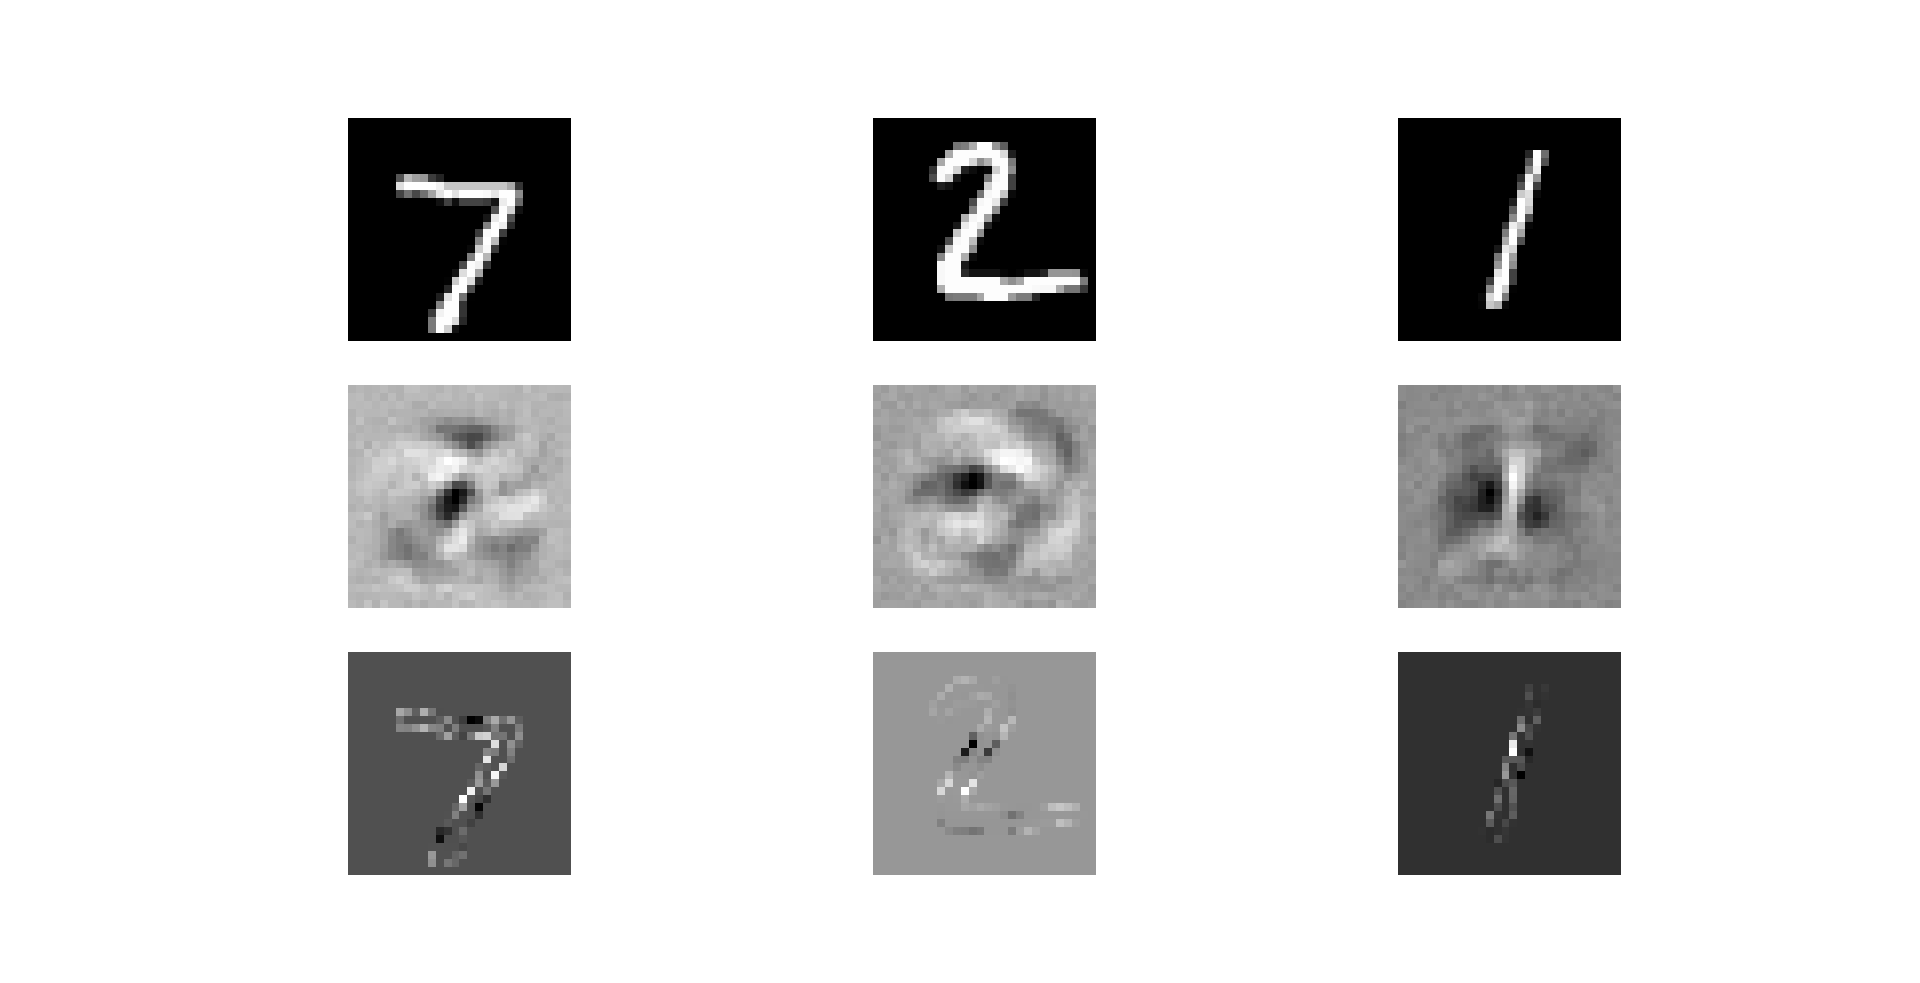
\includegraphics[width=\linewidth]{shapeshift.png}
	\caption{شکل و ماهیت حملات در صورت استفاده از توابع پایه‌ی تک‌جمله‌ای و چبیشف. ردیف بالا مثال‌های طبیعی، ردیف وسط شکل حمله در صورت استفاده از توابع پایه‌ی تک‌جمله‌ای و ردیف آخر ماهیت حمله در صورت استفاده از توابع پایه‌ی چبیشف را نشان می‌دهند.}
	\label{fig:shape}
\end{figure}

نکته‌ی دیگری که در شکل دیده می‌شود، مشابه بودن رفتار حمله در انتخاب جهت اختلال خصمانه است. با کمی دقت، به نظر می‌رسد پیکسل‌هایی که در دو حالت مشترک هستند، رفتار مشابهی نیز از خود نشان می‌دهند و در هر دو حالت مکان پیکسل در تصویر  شدت و علامت آن را تعیین می‌کند. این موضوع با نتیجه‌ای که در (مقاله) در مورد اهمیت جهت ورودی به دست آمده سازگاری دارد.

\section{جمع‌بندی}
در این مقاله دیدگاه جدیدی را در مورد چگونگی به وجود آمدن مثال‌های خصمانه و انتقال‌پذیری آنها در شبکه‌های عصبی را ارائه دادیم. طبق دیدگاه جدید، وجود مثال‌های خصمانه اثر جانبی پدیده‌ی رونگه و انتقال‌پذیری آنها نتیجه‌ی مستقیم اصل داربو است. پدیده‌ی رونگه هنگام درون‌یابی با استفاده از چندجمله‌ای‌هایی که همگرایی یکنواخت ندارند به وجود می‌آید. طبق نظریه‌ی تقریب جهانی، شبکه‌های عصبی توانایی تقریب زدن هر تابعی را دارند. با این حال، وجود مثال‌های خصمانه نشان می‌دهد که نوع همگرایی ساختار کنونی شبکه‌های عصبی به تابع مورد نظر یکنواخت نیست. در صورتی که همگرایی یکنواخت نباشد، خواص مهمی از شبکه‌های عصبی، از جمله پیوستگی، الزاما به تابع حدی منتقل نخواهند شد.

با توجه به این موضوع، برای غلبه بر مشکل مثال‌های خصمانه چند مسیر را می‌توان دنبال کرد. یک مسیر، جایگزین کردن توابع پایه‌ی تک‌جمله‌ای با توابع پایه‌ی چبیشف است. این تغییر باعث از میان رفتن مثال‌های خصمانه نمی‌شود و فقط پدیده‌ی رونگه را به پدیده‌ی گیبس تبدیل می‌کند. با این وجود، کاهش پدیده‌ی گیبس تاثیر مستقیمی بر مثال‌های خصمانه خواهد داشت.

مسیر دیگر، کاهش پدیده‌ی رونگه است. استفاده از گره‌های چبیشف به عنوان نقاط درون‌یابی یکی از اصلی‌ترین روش‌های کاهش تاثیر پدیده‌ی رونگه است. با این وجود، در این لحظه روش مستقیمی برای انتقال مفهوم گره‌های چبیشف به شبکه‌های عصبی موجود نیست. آموزش خصمانه ممکن است بتواند شبکه را به تمرکز بیشتر بر روی نواحی مرزی ترقیب کند ولی اثباتی در این مورد وجود ندارد.

مسیر سومی که در راستای حل مشکل مثال‌های خصمانه وجود دارد، ارائه‌ی ساخت جدیدی از شبکه‌های عصبی است که خاصیت همگرایی یکنواخت را داشته باشد. در درون‌یابی، این مسیر با موفقیت با استفاده از چندجمله‌ای‌های برنشتاین و خم‌های بزیر انجام شده است. طبق دیدگاه پیشنهادی، این مسیر بهترین نتیجه را به همراه خواهد داشت و پدیده‌ی مثال‌های خصمانه را از میان خواهد برد. با این وجود، این مسیر احتمالا نیازمند انجام تغییراتی بنیادی در ساخت شبکه‌های عصبی است.

در هر صورت، وجود مثال‌های خصمانه نشانگر نقصان دانش فعلی در مورد خواص و نوع همگرایی شبکه‌های عصبی است. تعیین نوع، دامنه و نرخ همگرایی شبکه‌های عصبی در مسائل مختلف  می‌تواند اطلاعات بیشتری را در مورد این خانواده از مدل‌ها ارائه دهد. همچنین، مشخص شدن این موارد تصویر کامل‌تری از ظرفیت‌های شبکه‌های عصبی و مشکلاتی که ممکن است هنگام استفاده‌ی آنها در کاربردهای مختلف پیش بیاید را در اختیار ما خواهد گذاشت.

\end{document}